\documentclass{article}
\usepackage[utf8]{inputenc}
\usepackage{hyperref,ragged2e,amsmath,multicol,setspace,
fancyhdr,amsfonts,tikz,pgfplots,nccmath,enumerate,verbatim}
\usepackage[a4paper, width=216mm, height=297mm, margin=3cm]{geometry}
\usepgfplotslibrary{polar,fillbetween}
\usepgflibrary{shapes.geometric}
\usetikzlibrary{calc,patterns,arrows}
\newcommand\mylog[1]{\mathop{{}^{#1}\mathrm{log}}}
\pgfplotsset{compat=1.15}
\pgfplotsset{my style/.append style={axis x line=middle, axis y line=
middle, xlabel={$x$}, ylabel={$y$}, axis equal }}
\usepackage{etoolbox}
\newcommand{\zerodisplayskips}{%
  \setlength{\abovedisplayskip}{0pt}%
  \setlength{\belowdisplayskip}{0pt}%
  \setlength{\abovedisplayshortskip}{0pt}%
  \setlength{\belowdisplayshortskip}{0pt}}
\pagestyle{fancy}
\fancyhf{}
\lhead{Halaman \thepage}
\rhead{Pembahasan Soal EAS 2021/2022 \\ (\href{https://instagram.com/ahmadzakiyudin_/}{@ahmadzakiyudin\_})}
\hypersetup{
    colorlinks=true,
    linkcolor=blue,
    filecolor=blue,      
    urlcolor=blue,
}
\setlength{\columnsep}{0.8cm}
\begin{document}
 \begin{titlepage}
    \vspace*{\fill}
    \begin{center}
      \Huge {PEMBAHASAN SOAL EAS \\ MATEMATIKA I \\ TAHUN 2021/2022}\\[0.4 cm]
      \huge {Ahmad Hisbu Zakiyudin}
    \end{center}
    \vspace*{\fill}
  \end{titlepage}
\makeatletter
\renewcommand*\env@matrix[1][*\c@MaxMatrixCols c]{%
  \hskip -\arraycolsep
  \let\@ifnextchar\new@ifnextchar
  \array{#1}}
\makeatother
\newcount\arrowcount
\newcommand\arrows[1]{
        \global\arrowcount#1
        \ifnum\arrowcount>0
                \begin{matrix}[c]
                \expandafter\nextarrow
        \fi
}
 
\newcommand\nextarrow[1]{
        \global\advance\arrowcount-1
        \ifx\relax#1\relax\else \xrightarrow{#1}\fi
        \ifnum\arrowcount=0
                \end{matrix}
        \else
                \\
                \expandafter\nextarrow
        \fi
}
\newpage
\setstretch{1.3}
\section*{SOAL SESI 1}
\begin{enumerate}
 
	\item Dapatkan 
	$$ \dfrac{d}{dx} \left[\sqrt{x^3+\csc x}\right] $$
	\textbf{Jawaban:}\\
	Ingat bahwa $\dfrac{d}{dx} x^n = nx^{n-1}$ dan $\dfrac{d}{dx} \csc x = -\cot x\csc x$. \\
	Ingat pula aturan rantai yaitu $\dfrac{d}{dx} [f(g(x))]=f'(g(x)) g'(x)$ sehingga diperoleh 
 	\begin{align*}
 	\dfrac{d}{dx} \left[\sqrt{x^3+\csc x}\right] = \dfrac{1}{2\sqrt{x^3+\csc x}}\times\left(3x^2-\cot x\csc x\right) = \dfrac{3x^2-\cot x\csc x}{2\sqrt{x^3+\csc x}}
 	\end{align*}
	\item Diberikan fungsi $f(x)=\dfrac{x+3}{x+2}$
	\begin{enumerate}
		\item Dapatkan $f'(x)$
		\item Jika $(x_0,y_0)$ titik pada kurva $f$,dapatkan titik $(x_0,y_0)$ dan garis singgung di titik $(x_0,y_0)$ yang tegak lurus dengan garis $y=x$.
	\end{enumerate}
	\textbf{Jawaban:}
	\begin{enumerate}
		\item Dapat dengan mudah diperoleh $y'=f'(x)=\dfrac{(x+2)(1)-(x+3)(1)}{(x+2)^2} = -\dfrac{1}{(x+2)^2}$
		\item Ingat bahwa gradien garis singgung kurva pada suatu titik pada kurva adalah nilai turunan pertama pada titik tersebut. Tinjau bahwa gradien garis singgung yang dimaksud tegak lurus dengan garis $y=x$ sehingga gradien garis singgungnya adalah $-1$. Selanjutnya kita cari nilai $x$ yang memenuhi $f'(x)=-1$
		\begin{align*}
		f'(x) = -\dfrac{1}{(x+2)^2} &= -1 \\
		(x+2)^2 &=1\\
		|x+2| &= 1 
		\end{align*}
		sehingga terdapat dua titik $x_0$ yang memenuhi, yaitu $x_0=-3$ dan $x_0=-1$. 
		\begin{enumerate}
			\item Untuk $x_0=-3$ kita peroleh $y_0=f(x_0)=f(-3)=0$ sehingga persamaan garis singgung di titik tersebut adalah 
			\begin{align*}
			y-y_0 &= m(x-x_0) \\
			y &= -1(x-(-3)) \\
			y &= -x-3 \\
			x+y +3&= 0
			\end{align*}
			\item Untuk $x_0=-1$, kita peroleh $y_0=f(x_0)=f(-1)=2$ sehingga persamaan garis singgung di titik tersebut adalah 
			\begin{align*}
			y-y_0 &= m(x-x_0)\\
			y-2 &= -1(x-(-1)) \\
			y &= -x+1 \\
			x+y-1 &= 0
			\end{align*}
		\end{enumerate}
		Jadi terdapat dua titik $(x_0,y_0)$ pada kurva $f(x)$ yang garis singgungnya tegak lurus dengan garis $y=x$, yaitu titik $(-3,0)$ dengan garis singgung $x+y+3=0$ dan titik $(-1,2)$ dengan garis singgung $x+y-1=0$
	\end{enumerate}
	\item Tentukan nilai maksimum dan minimum dari fungsi 
	$$f(x)=\begin{cases} 4x-1, &x<1 \\
	x^2-3x+5, &x\geq 1\end{cases}$$ 
	pada $\left[\frac{2}{3},\frac{5}{3}\right]$
	\\[0.1 cm] \textbf{Jawaban:}\\
	Akan kita cari masing-masing nilai maksimum dan minimum $f(x)$ pada selang $\left[\frac{2}{3},1\right)$ dan $\left[1,\frac{5}{3}\right]$
	\begin{enumerate}
		\item[i.] Untuk selang $\left(\frac{2}{3},1\right)$, diperoleh $f(x)=4x-1$ dan $f'(x)=4$, sehingga $f'(x)>0$ untuk setiap $x$ pada selang tersebut, serta $f(x)$ tidak memiliki titik stasioner. Oleh karena itu, dapat dicek pada batas selangnya, yaitu $f\left(\frac{2}{3}\right)=\dfrac{5}{3}$ adalah nilai minimum. Sedangkan nilai maksimumnya tidak ada, tetapi mendekati $\displaystyle \lim_{x\rightarrow 1^-} 4x-1 = 3$.
		\item[ii.] Untuk selang $\left(1,\frac{5}{3}\right)$, diperoleh $f(x)=x^2-3x+5$ dan $f'(x)=2x-3$. Dapat diperoleh pula $f''(x)=2$ sehingga $f''\left(\frac{3}{2}\right)=2>0$, artinya $x=\dfrac{3}{2}$ merupakan nilai minimum relatif. Selanjutnya dapat dicek nilai $f(x)$ pada batas selang dan titik stasioner 
		\begin{align*}
		f(1)&=1^2-3(1)+5=3 \\
		f\left(\frac{3}{2}\right) &=\left(\frac{3}{2}\right)^2-3\left(\frac{3}{2}\right) +5 = \frac{11}{4} \\
		f\left(\frac{5}{3}\right) &= \left(\frac{5}{3}\right)^2-3\left(\frac{5}{3}\right)+5 = \frac{25}{9}
		\end{align*}
		sehingga nilai minimum pada selang $\left[1,\frac{5}{3}\right]$ adalah $f\left(\frac{3}{2}\right) = \frac{11}{4}$ dan maksimum adalah $f(1)=3$
	\end{enumerate}
	Apabila kedua hasil tersebut digabungkan, dapat diperoleh nilai maksimum dan minimum global berturut-turut $f(1)=3$ dan $f\left(\frac{2}{3}\right) = \frac{5}{3}$. Selain itu, diperoleh pula maksimum relatif dan minimum relatif berturut-turut $f\left(\frac{5}{3}\right)=\frac{25}{9}$ dan $f\left(\frac{3}{2}\right)=\frac{11}{4}$\
 
	\newpage 
	\item Dapatkan ukuran silinder/tabung dengan isi maksimum yang dapat dibuat dalam bola berjari-jari 100 cm.\\
	\textbf{Jawaban:}\\
	Misalkan jari-jari tabung adalah $a$, maka untuk mencari tingginya, kita dapat membuat proyeksi 2 dimensi untuk tabung dalam bola. Proyeksinya akan berbentuk seperti persegi panjang dalam lingkaran berikut
	\begin{center}
	\begin{tikzpicture}[scale=0.8]
		\begin{axis}[
x = 1 cm, y=1 cm,
 axis lines=middle,
  xmin=-5,xmax=5,ymin=-5,ymax=5,
  ticks=none,
  yticklabels={,,},
  xlabel=$x$,
  ylabel=$y$]
\draw (0,0) circle(4);
\fill (3.266,2.3094) circle(2pt) node[right] {\large{$(a,b)$}};
\draw[dashed] (0,0) -- (3.266,2.3094);
\draw[dashed] (-3.266,2.3094) rectangle (3.266,-2.3094);
\node [rotate=35.3] at (1.3,1.3) {\large{$R$}};
\end{axis}
\end{tikzpicture}
	\end{center}	
 Tanpa mengurangi keumuman, misalkan pusat lingkaran adalah $(0,0)$ dan jari-jarinya sama seperti jari-jari bola, yaitu $R$ sehingga dapat diperoleh persamaan lingkaran $x^2+y^2=R^2$. Selanjutnya, karena jari-jari tabung adalah $a$, maka $a^2+y^2=R^2$. Misalkan pula titik $(a,b)$ melewati lingkaran, sehingga tinggi tabungnya adalah $2b$. Jadi kita punya $a^2+b^2=R^2$ atau $a^2=R^2-b^2$. Oleh karena itu diperoleh volume tabung
	$$ V = \pi a^2(2b) = 2\pi (R^2-b^2)b = 2\pi(R^2b-b^3) $$
	 Volume terbesar atau maksimum ketika $\dfrac{dV}{db}=0$, yaitu
	 \begin{align*}
	 \dfrac{dV}{db} = 2\pi (R^2-3b^2) &= 0 \\
	 (R-b\sqrt{3})(R+b\sqrt{3}) &=0
	 \end{align*}
	 Karena $b>0$, diperoleh $b=\dfrac{R}{3}\sqrt{3}$ sehingga $a^2=\dfrac{2R^2}{3}$. Dengan kata lain ukuran jari-jari tabung yaitu $a=\dfrac{R}{3}\sqrt{6}$ dan tingginya adalah $2b=\dfrac{2R}{3}\sqrt{3}$, serta volumenya adalah $V=2\pi \left(R^2\dfrac{R}{3}\sqrt{3}-\left(\dfrac{R}{3}\sqrt{3}\right)^3\right) = \dfrac{4\pi R^3\sqrt{3}}{9}$.\\
 	Karena $R=100~ cm=1~ m$, diperoleh $V=\dfrac{4\pi \sqrt{3}}{9} ~m^3$.
 	\newpage
	\item Selesaikan integral $\int_0^{2\pi} |\cos x|~ dx$\\
	\textbf{Jawaban:}\\
	Tinjau bahwa 
	\begin{align*}
	|\cos x| = \begin{cases}
	\cos x, \quad &0\leq x\leq \frac{\pi}{2} \vee \frac{3\pi}{2} \leq x\leq 2\pi\\
	-\cos x, \quad & \frac{\pi}{2}< x< \frac{3\pi}{2}
	\end{cases}
	\end{align*}
	sehingga integralnya menjadi 
	\begin{align*}
	\int_0^{2\pi} |\cos x| ~ dx &= \int_0^{\frac{\pi}{2}} \cos x~ dx + \int_{\frac{3\pi}{2}}^{2\pi} \cos x ~dx + \int_{\frac{\pi}{2}}^{\frac{3\pi}{2}} (-\cos x)~ dx\\
	&= \sin x|_0^{\frac{\pi}{2}} + \sin x|_{\frac{3\pi}{2}}^{2\pi} -\sin x|_{\frac{\pi}{2}}^{\frac{3\pi}{2}}\\
	&= 1-0 + 0-(-1) - (-1-1) = 4
	\end{align*}
\end{enumerate}
\newpage
\section*{SOAL SESI 2}
\begin{enumerate}
	\item Jika $y=\sqrt{3x+\sin 4x^2}$ dapatkan $\dfrac{dy}{dx}=\cdots$\\
	\textbf{Jawaban:}\\
	Ingat bahwa $\dfrac{d}{dx} x^n = nx^{n-1}$ dan $\dfrac{d}{dx} \sin x = \cos x$. \\
	Ingat pula aturan rantai yaitu $\dfrac{d}{dx} [f(g(x))]=f'(g(x)) g'(x)$ sehingga diperoleh 
 	\begin{align*}
 	\dfrac{dy}{dx} \sqrt{3x+\sin 4x^2} &= \dfrac{1}{2\sqrt{3x+\sin 4x^2}}\times [3+(\cos 4x^2)\times (8x)] = \dfrac{3+8x\cos 4x^2}{2\sqrt{3x+\sin 4x^2}}
 	\end{align*}
	\item Diketahui $f(x)=1+|x+2|$. Tunjukkan apakah $f(x)$ dapat diturunkan di $x=-2$?\\
	\textbf{Jawaban:}\\
	Perhatikan bahwa $f(x)=\begin{cases}1+x+2,\qquad &x\geq -2\\
	1-x-2,\qquad &x< -2\end{cases}$. Dapat diperoleh bahwa 
	\begin{align*}
	f'_-(-2) &= \lim_{h\rightarrow 0} \dfrac{1-(-2+h)-2-(1-(-2)-2)}{h} = \lim_{h\rightarrow 0} \dfrac{-h}{h} = -1\\
	f'_+(-2) &= \lim_{h\rightarrow 0} \dfrac{1+(-2+h)+2-(1+(-2)+2)}{h} =\lim_{h\rightarrow 0} \dfrac{h}{h} = 1
	\end{align*}
	Jelas bahwa $f'_-(-2) \neq f'_+(-2)$ sehingga $f(x)$ tidak dapat diturunkan di $x=-2$.
	\item Diberikan $f(x)=\dfrac{x^3}{x^2+1}$
	\begin{enumerate}
		\item Tentukan asimtot datar, tegak dan miring (jika ada)
		\item Tentukan selang fungsi naik/turun dan titik stasioner (titik maksimum/minimum) (jika ada)
		\item Tentukan selang kecekungan fungsi dan titik belok (jika ada)
		\item Sketsa grafik fungsi
	\end{enumerate}
	\textbf{Jawaban:}
	\begin{enumerate}
		\item Suatu fungsi $f(x)=\dfrac{p(x)}{q(x)}$ memiiki asimtot datar jika $\displaystyle \lim_{x\rightarrow \infty} f(x) = b$.\\ Jika $p(x)$ dan $q(x)$ polinomial, maka $f(x)$ memiliki asimtot datar jika pangkat tertinggi dari $p(x)$ dan $q(x)$ sama. Karena pangkat tertinggi dari $p(x)$ berbeda dengan pangkat tertinggi dari $q(x)$, maka $f(x)$ tidak memiliki asimtot datar. \\
		Untuk asimtot tegak, $x=a$ disebut asimtot tegak dari fungsi $f(x)$ jika $\displaystyle \lim_{x\rightarrow a} f(x)=\infty$. \\
		Jika $f(x)=\dfrac{p(x)}{q(x)}$, maka $f(x)$ memiliki asimtot tegak $x=a$ jika $q(a)=0$. Karena $q(x)=x^2+1\geq 1$, maka $q(x)\neq 0$ untuk setiap $x\in \mathbb{R}$ sehingga $f(x)$ tidak memiliki asimtot tegak.\\
		Untuk asimtot miring dari suatu fungsi $f(x)=\dfrac{p(x)}{q(x)}$ yang dapat dinyatakan sebagai $f(x)=(ax+b)+\dfrac{r(x)}{q(x)}$, maka $y=ax+b$ merupakan asimtot miring dari $f(x)$.\\
		Perhatikan bahwa $f(x)=\dfrac{x^3}{x^2+1} = \dfrac{x^3+x-x}{x^2+1} = x-\dfrac{x}{x^2+1}$.
		Diperoleh asimtot miringnya adalah $y=x$.
		\item Tinjau bahwa 
		\begin{align*}
		f'(x) &= \dfrac{3x^2(x^2+1)-2x(x^3)}{x^2+1}\\
		&=\dfrac{x^4+3x^2}{x^2+1}\\
		&= \dfrac{x^2(x^2+3)}{(x^2+1)^2}
		\end{align*}
		Karena $x^2+3\geq 3$, maka $f'(x)=0$ jika $x=0$. Diperoleh titik kritisnya adalah $(0,f(0))=(0,0)$. \\		
		Kemudian perhatikan bahwa $f'(x)=\dfrac{x^4+3x^2}{(x^2+1)^2} \geq 0$ untuk setiap $x\in\mathbb{R}$ sehingga $f(x)$ naik untuk setiap $x\in\mathbb{R}$. Hal ini mengakibatkan titik $(0,0)$ bukan titik stasioner.
		\item Tinjau bahwa 
		\begin{align*}
		f''(x) &= \dfrac{(4x^3+6x)(x^2+1)^2-2(x^2+1)(2x)(x^4+3x^2)}{(x^2+1)^4}\\
		&= \dfrac{(4x^3+6x)(x^2+1)-4x(x^4+3x^2)}{(x^2+1)^3}\\
		&= \dfrac{4x^5+10x^3+6x-4x^5-12x^3}{(x^2+1)^3}\\
		&=\dfrac{-2x^3+6x}{(x^2+1)^3}\\
		&= \dfrac{-2x(x^2-3)}{(x^2+1)^3}\\
		&= \dfrac{-2x(x-\sqrt{3})(x+\sqrt{3})}{(x^2+1)^3}
		\end{align*}
		Karena $x^2+1\geq 1$, maka $f''(x)=0$ jika $x=0$ atau $x=\pm \sqrt{3}$. \\
		Dengan uji titik, diperoleh 
		\begin{center}
		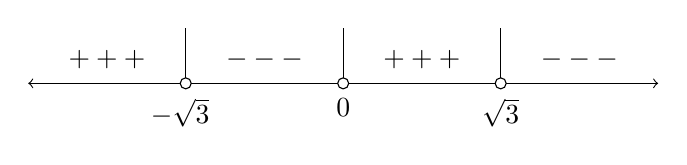
\begin{tikzpicture}
	\draw[<-] (0,0) -- (2-0.07,0);
	\draw (2+0.07,0) -- (4-0.07,0);
	\draw (4+0.07,0) -- (6-0.07,0);
	\draw[->] (6+0.07,0) -- (8,0);
	\draw (2,0.07) -- (2,0.7);
	\draw (4,0.07) -- (4,0.7);
	\draw (1,0.3) node {$+++$};
	\draw (3,0.3) node {$---$};
	\draw (7,0.3) node {$---$};
	\draw (5,0.3) node {$+++$};
	\draw (2,0) circle(0.07);
	\draw (4,0) circle(0.07);
	\draw (2-0.07,-0.07) node[below] {$-\sqrt{3}$};
	\draw (4,-0.07) node[below] {$0$};
	\draw (6,-0.07) node[below] {$\sqrt{3}$};
	\draw (6,0) circle(0.07);
	\draw (6,0.07) -- (6,0.7);
	\end{tikzpicture}
		\end{center}
		Didapatkan bahwa $f(x)$ cekung ke atas pada selang $(-\infty,-\sqrt{3})~\bigcup ~(0,\sqrt{3})$ karena $f''(x)> 0$ pada selang tersebut. Didapatkan pula $f(x)$ cekung ke bawah pada selang $(-\sqrt{3},0)~\bigcup ~(\sqrt{3},+\infty)$ karena $f''(x)< 0$ pada selang tersebut.\\
		Karena $f''(x)$ berubah tanda pada $x=0$ dan $x=\pm \sqrt{3}$, maka $(0,f(0)), (-\sqrt{3},f(-\sqrt{3})),$ dan $(\sqrt{3},f(\sqrt{3}))$ merupakan titik belok dari $f(x)$.
		\item Didapatkan sketsa grafik fungsinya adalah 
		\begin{center}
		\begin{tikzpicture}
\begin{axis}[
x= 0.7 cm, y=0.7 cm,
 axis lines=middle,
  xmin=-7.3,xmax=7.3,ymin=-7.3,ymax=7.3,
  xtick distance=1,
  ytick distance=1,
  xlabel=$x$,
  ylabel=$y$]
\addplot [domain=-6.5:6.5, samples=250, blue] {x*x*x/(x*x+1)};
\addplot [domain=-6.5:6.5,dashed]{x};
\end{axis}
\end{tikzpicture}
		\end{center}
	\end{enumerate}
 
	\item Tentukan tinggi dan jari-jari kerucut lingkaran tegak dengan isi minimum yang dibatasi bola berjari-jari $R$.\\
	\textbf{Jawaban:}\\
	Kalimat dari soal ini sebenarnya sedikit membingunkan, karena jika kerucut di dalam bola, maka volumenya minimumnya dapat dibuat 0. Soal ini akan dikerjakan dengan asumsi kerucut di luar bola.
 	Misalkan jari-jari kerucut adalah $r$, maka untuk mencari tingginya, kita dapat membuat proyeksi 2 dimensi untuk bola di dalam kerucut.
	\begin{center}
	\begin{tikzpicture}[scale=1]
\draw (0,0) circle(2);
\fill (0,4) circle(2pt);
\fill (-3.46,-2) circle(2pt);
\fill (3.46,-2) circle(2pt);
\draw[dashed] (0,0) -- (1.73,1);
\draw (0,4) -- (-3.46,-2) -- (3.46,-2) -- (0,4);
\draw[dashed] (0,-2) -- (0,4); 
\node at (0,4.4) {\large{$A$}};
\node at (-3.6,-2.4) {\large{$B$}};
\node at (-0.3,0.2) {\large{$O$}};
\fill (0,-2) circle(2pt);
\fill (1.73,1) circle(2pt);
\fill (0,0) circle(2pt);
\node at (2,1.1) {\large{$Q$}};
\node at (0,-2.4) {\large{$P$}};
\node at (3.6,-2.4) {\large{$C$}};
\draw (0.2,-2) -- (0.2,-1.8) -- (0,-1.8);
\draw (1.65,1.15) -- (1.5,1.06) -- (1.58,0.91);
\end{tikzpicture}
	\end{center}
	Misalkan $AP=H$, $PC=r$, dan $OP=R$, maka $AO=H-R$ dengan $H>2R$ dan diperoleh 
	\begin{align*}
	\sin (\angle PAC) = \dfrac{OQ}{AO} &= \dfrac{PC}{AC}\\
	\dfrac{R}{H-R} &= \dfrac{r}{\sqrt{r^2+H^2}}\\
	\dfrac{R^2}{(H-R)^2} &= \dfrac{r^2}{r^2+H^2}\\
	R^2(r^2+H^2)&=r^2(H^2-2RH+R^2)\\
	\dfrac{R^2H^2}{H^2-2RH} &= r^2\\
	r^2 &= \dfrac{R^2H}{H-2R}
	\end{align*}
	Selanjutnya volume kerucutnya adalah
	\begin{align*}
	V &= \dfrac{\pi}{3}r^2H\\
	&= \dfrac{\pi}{3}\left(\dfrac{R^2H^2}{H-2R}\right)
	\end{align*}
	Akan minimum jika $\dfrac{dV}{dH}=0$ sehingga
	\begin{align*}
	\dfrac{dV}{dH} &= \dfrac{\pi}{3}\left(\dfrac{2HR^2(H-2R)-R^2H^2}{(H-2R)^2}\right)\\
	&= \dfrac{R^2H^2-4HR^3}{(H-2R)^2}\\
	0 &= \dfrac{R^2H(H-4R)}{(H-2R)^2}\\
	0 &= H-4R\\
	H &= 4R
	\end{align*}
	Dengan demikian tingginya adalah $H=4R$ serta jari-jarinya adalah $r=\sqrt{\dfrac{R^2(4R)}{4R-2R}} = R\sqrt{2}$.
	\item Hitunglah integral berikut 
	$$ \int_0^4 \dfrac{x-2}{\sqrt{x^2-4x+7}}~ dx $$
	[Petunjuk: gunakan $u=x-2$].\\
	\textbf{Jawaban:}\\
	Misalkan $u=x-2$ sehingga $du = dx$, selanjutnya, kita punya 
	\begin{align*}
	\int \dfrac{x-2}{\sqrt{x^2-4x+7}} \, dx = \int \dfrac{x-2}{(x-2)^2+3}\, dx = \int \dfrac{u}{\sqrt{u^2+3}}\, du
	\end{align*}
	Misalkan $u^2+3=p$ sehingga $2u \, du = dp$, diperoleh 
	\begin{align*}
	\int \dfrac{u}{\sqrt{u^2+3}} \, du = \int \dfrac{2}{\sqrt{p}}\, dp = \int 2p^{-1/2} \, dp = 2(2)p^{1/2} = 4\sqrt{p}
	\end{align*}
	Dengan demikian 
	\begin{align*}
	\int_0^4 \dfrac{x-2}{\sqrt{x^2-4x+7}}\, dx = 4\sqrt{p}\bigg|^{x=4}_{x=0} &= 4\sqrt{u^2+3}\bigg|^{x=4}_{x=0} \\
	&= 4\sqrt{x^2-4x+7}\bigg|^4_0 = 4(\sqrt{7}-\sqrt{7}) = 0
	\end{align*}
	\textbf{Alternatif Jawaban:}\\
	Misalkan $u=x-2$ sehingga $du=dx$ serta batas atasnya adalah $u=4-2=2$ dan batas bawahnya $u=0-2=-2$, diperoleh 
	\begin{align*}
	\int_0^4 \dfrac{x-2}{\sqrt{x^2-4x+7}}\, dx = \int_{-2}^2 \dfrac{u}{\sqrt{u^2+3}} \, du
	\end{align*}
	Perhatikan bahwa jika $f(u)=\dfrac{u}{\sqrt{u^2+3}}$, maka 
	$$f(-u)=\dfrac{-u}{\sqrt{(-u)^2+3}}=-\dfrac{u}{\sqrt{u^2+3}}=-f(u)$$ sehingga $f(u)$ fungsi ganjil. Dengan demikian
	\begin{align*}
	\int_{-2}^2 f(u) \, du = 0
	\end{align*}
\end{enumerate}
\newpage
\section*{SOAL SESI 3}
\textbf{Catatan:} Untuk soal no 1 dan 2, nilai $a$ dan $b$ diambil dari dua digit terakhir NRP Anda. \\
Sebagai contoh jika NRP Anda adalah 5002201148 maka $a=4$ dan $b=8$.\\
Namun jika $a$ atau $b$ bernilai 0, maka ganti dengan angka 10
\begin{enumerate}
	\item Suatu titik $P$ bergerak sepanjang kurva dengan persamaan $y=\sqrt{ax+b^2}$. Selanjutnya, didefinisikan $l$ sebagai jarak titik $P$ terhadap titik $(2,0)$. Dengan asumsi bahwa $x$ bertambah dengan laju 4 satuan/det pada saat $x=3$
	\begin{enumerate}
		\item Dengan laju berapakah $l$ berubah saat itu?
		\item Apakah $l$ berkurang atau bertambah saat itu?
	\end{enumerate}
	\textbf{Jawaban:}\\
	Ingat jarak suatu titik $(x_0,y_0)$ ke titik $(x,y)$ adalah $l=\sqrt{(x-x_0)^2+(y-y_0)^2}$. Dalam hal ini $x_0=2,y_0=0$ sehingga $l=\sqrt{(x-2)^2+y^2}$. Karena $y=\sqrt{4x+64}$, maka $$l=\sqrt{x^2-4x+4+4x+64}=\sqrt{x^2+68}$$
	\begin{enumerate}
		\item Dari soal, kita punya $\dfrac{dx}{dt}\bigg|_{x=3} = 4$ sehingga 
		\begin{align*}
		\dfrac{dl}{dt} &= \dfrac{2x}{2\sqrt{x^2+68}}\dfrac{dx}{dt}\\
		&= \dfrac{3}{\sqrt{9+68}}\times 4\\
		&= \dfrac{12}{\sqrt{77}}
		\end{align*}
	Jadi $l$ berubah dengan laju $\dfrac{12}{\sqrt{77}}$
	\item Karena $\dfrac{12}{\sqrt{77}}>0$, maka $l$ bertambah pada saat itu.
	\end{enumerate}
	\item Diketahui garis singgung kurva $ay^3=bx^2$ di titik $(x_0,y_0)$ sejajar dengan garis $2x+3y=5$.
	\begin{enumerate}
		\item Dapatkan titik $(x_0,y_0)$
		\item Dapatkan persamaan garis singgung di titik $(x_0,y_0)$ yang telah diperoleh 
	\end{enumerate}
	\textbf{Jawaban:}
	\begin{enumerate}
		\item Perhatikan bahwa persamaan garis $2x+3y=5$ dapat diubah menjadi bentuk $y=mx+c$ dengan $m$ adalah gradiennya. Diperoleh $y=-\dfrac{2}{3}x+\dfrac{5}{3}$ sehingga gradiennya adalah $-\dfrac{2}{3}$. Karena garis singgungnya sejajar, maka gradiennya sama. \\
		Selanjutnya, ingat bahwa gradien garis singgung kurva pada suatu titik $(x_0,y_0)$ adalah nilai turunan pertama persamaan kurva tersebut pada titik $(x_0,y_0)$.\\
		Tinjau bahwa persamaan kurvanya adalah $4y^3=8x^2$ atau $y=(2x^2)^{1/3}$. Diperoleh 
		\begin{align*}
		\dfrac{dy}{dx} &= \dfrac{1}{3}(2x^2)^{-2/3}\times 4x\\
		&= \dfrac{4x}{3(2x^2)^{2/3}}\\
		-\dfrac{2}{3} &= \dfrac{4x}{3(2x^2)^{2/3}}\\
		-(2x^2)^{2/3} &= 2x\\
		-(2x^2)^2 &= 8x^3\\
		-4x^4 -8x^3 &= 0\\
		-4x^3(x+2) &= 0
		\end{align*}
		Karena $\dfrac{dy}{dx}$ tak terdefinisi saat $x=0$, maka $x_0=-2$ dan diperoleh $y_0=2$.
	\end{enumerate}
	\item Diberikan $f(x)=x^{5/3}-5x^{2/3}$
	\begin{enumerate}
		\item Tentukan titik stasioner (titik maksimum/minimum relatif) jika ada
		\item Tentukan selang kecekungan fungsi dan titik belok jika ada
		\item Sketsa grafik fungsi
	\end{enumerate}
	\textbf{Jawaban:}
	\begin{enumerate}
		\item Untuk menentukan titik stasioner, tinjau 
		\begin{align*}
		f'(x) &= 	\dfrac{5}{3}x^{2/3} -\dfrac{10}{3}x^{-1/3} \\
		&= \dfrac{5}{3}\left(x^{2/3} -\dfrac{2}{x^{1/3}}\right) \\
		&= \dfrac{5}{3}\left(\dfrac{x-2}{x^{1/3}}\right) 
		\end{align*}
		Diperoleh titik kritisnya adalah $x=0$ dan $x=2$. Dengan uji titik, didapatkan 
		\begin{center}
		\begin{tikzpicture}
	\draw[<-] (0,0) -- (2-0.07,0);
	\draw (2+0.07,0) -- (4-0.07,0);
	\draw[->] (4+0.07,0) -- (6,0);
	\draw (2,0.07) -- (2,0.7);
	\draw (4,0.07) -- (4,0.7);
	\draw (1,0.3) node {$+++$};
	\draw (3,0.3) node {$---$};
	\draw (5,0.3) node {$+++$};
	\draw (2,0) circle(0.07);
	\draw (4,0) circle(0.07);
	\draw (2,-0.07) node[below] {$0$};
	\draw (4,-0.07) node[below] {$2$};
	\end{tikzpicture}
		\end{center}
		Karena $f(x)$ kontinu di titik $x=0$ dan titik $x=2$, serta terjadi perubahan tanda dari positif ke negatif di titik $x=0$ dan dari negatif ke positif di titik $x=2$, maka titik $(0,f(0))=(0,0)$ merupakan titik maksimum relatif dan titik $(2,f(2))=(2,2^{5/3}-5(2)^{2/3})$ merupakan titik minimum relatif.
		\item Tinjau 
		\begin{align*}
		f''(x) &= \dfrac{5}{3}\left(\dfrac{2}{3}x^{-1/3}+\dfrac{2}{3}x^{-4/3}\right)\\
		&= \dfrac{10}{9}\left(\dfrac{1}{x^{1/3}}+\dfrac{1}{x^{4/3}}\right)\\
		&= \dfrac{10}{9}\left(\dfrac{x+1}{x^{4/3}}\right)
		\end{align*}
		Uji titik untuk $x=0$ dan $x=-1$, diperoleh 
		 \begin{center}
		\begin{tikzpicture}
	\draw[<-] (0,0) -- (2-0.07,0);
	\draw (2+0.07,0) -- (4-0.07,0);
	\draw[->] (4+0.07,0) -- (6,0);
	\draw (2,0.07) -- (2,0.7);
	\draw (4,0.07) -- (4,0.7);
	\draw (1,0.3) node {$---$};
	\draw (3,0.3) node {$+++$};
	\draw (5,0.3) node {$+++$};
	\draw (2,0) circle(0.07);
	\draw (4,0) circle(0.07);
	\draw (2,-0.07) node[below] {$-1$};
	\draw (4,-0.07) node[below] {$0$};
	\end{tikzpicture}
		\end{center}
		Dari sini diperoleh $f(x)$ cekung ke bawah pada selang $(-\infty,-1)$ dan cekung ke atas pada $(-1,0)\cup (0,+\infty)$. \\
		Kemudian karena $f(x)$ kontinu di titik $x=-1$ dan $f''(x)$ hanya berubah tandanya di $x=-1$, maka titik beloknya hanyalah $(-1,f(-1))=(-1,-6)$
		\item Diperoleh sketsa grafiknya
		\begin{center}
		\begin{tikzpicture}
		[
    declare function=
    {
      t(\x) = x/abs(x)*(abs(\x))^(1/3) ;
    }
  ]
\begin{axis}[
x =.6 cm, y=.5 cm,
 axis lines=middle,
  xmin=-3.5,xmax=7.5,ymin=-12,ymax=5.5,
  xtick distance=1,
  ytick distance=1,
  xlabel=$x$,
  ylabel=$y$]
\addplot [blue,domain=-2:7, samples=5000] {t(x)^5-5*t(x)^2};
\end{axis}
\end{tikzpicture}
		\end{center}
	\end{enumerate}
	\item Trapesium dilukiskan dalam setengah lingkaran berjari-jari 3 sehingga satu sisi berada pada diameternya, seperti pada gambar berikut.
	\begin{center}
	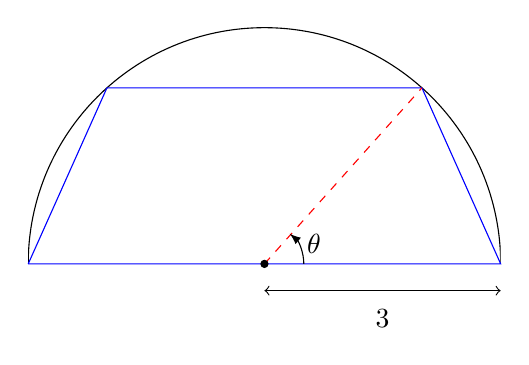
\begin{tikzpicture}
	\begin{scope}
    \clip (-3,0) rectangle (3,3);
    \draw (0,0) circle(3);
	\end{scope}
	\draw[blue] (-3,0) -- (-2,2.236) -- (2,2.236) -- (3,0) -- (-3,0);
	\draw[red,dashed] (0,0) -- (2,2.236);
	\fill (0,0) circle(1.5pt);
	\draw[<->] (0,-0.34) -- (3,-0.34);
	\draw (1.5,-0.7) node {3};
	\draw[-latex] (0:0.5) arc (0:50:0.5) ;
	\draw (0.63,0.26) node {$\theta$};
	\end{tikzpicture}
	\end{center}
	Tentukan luas maksimum trapesium [petunjuk: ekspresikan luas trapesium dalam bentuk $\theta$].\\
	\textbf{Jawaban:}\\
	Perhatikan bahwa trapesium tersebut dapat dibagi menjadi 3 bagian seperti berikut
	\begin{center}
	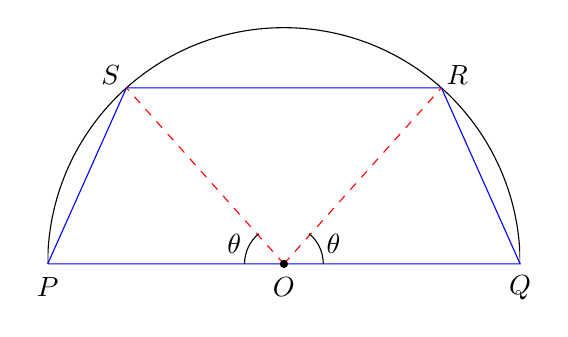
\begin{tikzpicture}
	\begin{scope}
    \clip (-3,0) rectangle (3,3);
    \draw (0,0) circle(3);
	\end{scope}
	\draw[blue] (-3,0) -- (-2,2.236) -- (2,2.236) -- (3,0) -- (-3,0);
	\draw[red,dashed] (0,0) -- (2,2.236);
	\draw[red,dashed] (0,0) -- (-2,2.236);
	\fill (0,0) circle(1.5pt);
	\draw (0:0.5) arc (0:50:0.5);
	\draw (0.63,0.26) node {$\theta$};
	\draw (-0.5,0) arc (180:130:0.5);
	\draw (-0.63,0.26) node {$\theta$};
	\draw (-3,-0.3) node{$P$};
	\draw (3,-0.3) node{$Q$};
	\draw (2.2,2.4) node{$R$};
	\draw (0,-0.3) node{$O$};
	\draw (-2.2,2.4) node{$S$};
	\end{tikzpicture}
	\end{center}
	Didapatkan $OP=OQ=OR=OS=3$, $\angle QOR = \angle POS = \theta$, dan $\angle SOR = \pi -2\theta$ dengan $0<\theta<\pi$.
	Dari sini, kita punya 
	$$ L_{PQRS} = L_{ROQ} + L_{SOR} + L_{POS}$$
	Dengan aturan sinus, maka
	\begin{align*}
	L_{PQRS} &= \dfrac{1}{2}(OQ)(OR)(\sin \angle QOR)+\dfrac{1}{2}(OR)(OS)(\sin\angle SOR)+\dfrac{1}{2}(OS)(OP)(\sin \angle POS)\\
	&= \dfrac{1}{2}\left(9\sin\theta+9\sin(\pi-2\theta)+9\sin \theta\right)\\
	&= \dfrac{1}{2}\left(18\sin\theta+9\sin 2\theta\right)
	\end{align*}
	Luas trapesium tersebut akan maksimum jika $\dfrac{dL}{d\theta} = 0$, sehingga
	\begin{align*}
	\dfrac{dL}{d\theta} &= 9\cos\theta +9\cos 2\theta \\
	0 &= \cos\theta + 2\cos^2\theta -1 \\
	0 &= (\cos \theta +1)(2\cos\theta-1)
	\end{align*}
	Karena $0<\theta<\pi$, maka $\cos\theta+1\neq 0$ sehingga haruslah $2\cos\theta-1=0$ atau $\cos\theta=\dfrac{1}{2}$.\\
	Didapatkan $\sin\theta=\dfrac{1}{2}\sqrt{3}$ serta luas maksimumnya adalah 
	\begin{align*}
	L_{PQRS} &= \dfrac{1}{2}(18\sin \theta+18\sin\theta\cos\theta)\\
	&= 9\times\dfrac{1}{2}\sqrt{3}+9\times\dfrac{1}{2}\sqrt{3}\times\dfrac{1}{2}\\
	&= \dfrac{27}{4}\sqrt{3}
	\end{align*}
	\item Misal $F(x)=\displaystyle \int_0^x \dfrac{2t-3}{4t^2+7}~ dt$ untuk $-\infty <x<+\infty$
	\begin{enumerate}
		\item Dapatkan interval di mana $F$ naik dan $F$ turun.
		\item Dapatkan interval di mana $F$ cekung ke atas dan $F$ cekung ke bawah.
	\end{enumerate}
	\textbf{Jawaban:}
	\begin{enumerate}
		\item Dengan teorema fundamental kalkulus 2, diperoleh 
		\begin{align*}
		F'(x) = \dfrac{2x-3}{4x^2+7}
		\end{align*}
		Karena penyebutnya $4x^2+7\geq 7$, titik kritisnya hanyalah $x=\dfrac{3}{2}$. Untuk selang $(-\infty,\frac{3}{2}]$, diperoleh $F'(x)\leq 0$ sehingga turun pada selang tersebut. Sedangkan untuk selang $[\frac{3}{2},+\infty)$, diperoleh $F'(x)\geq 0$ sehingga naik pada selang tersebut.
		\item Tinjau 
		\begin{align*}
		F''(x) &= \dfrac{2(4x^2+7)-(2x-3)(8x)}{(4x^2+7)^2}\\
		&= \dfrac{-8x^2+24x+14}{(4x^2+7)^2}\\
		&= \dfrac{-2(2x-7)(2x+1)}{(4x^2+7)^2}
		\end{align*}
		Uji titik untuk $x=-\dfrac{1}{2}$ dan $x=-\dfrac{7}{2}$, diperoleh
		\begin{center}
		\begin{tikzpicture}
	\draw[<-] (0,0) -- (2-0.07,0);
	\draw (2+0.07,0) -- (4-0.07,0);
	\draw[->] (4+0.07,0) -- (6,0);
	\draw (2,0.07) -- (2,0.7);
	\draw (4,0.07) -- (4,0.7);
	\draw (1,0.3) node {$---$};
	\draw (3,0.3) node {$+++$};
	\draw (5,0.3) node {$---$};
	\draw (2,0) circle(0.07);
	\draw (4,0) circle(0.07);
	\draw (2,-0.07) node[below] {$-\dfrac{1}{2}$};
	\draw (4,-0.07) node[below] {$\dfrac{7}{2}$};
	\end{tikzpicture}
		\end{center}
		Dari sini diperoleh bahwa $F(x)$ cekung ke bawah pada selang $(-\infty,-\frac{1}{2})\cup (\frac{7}{2},+\infty)$ serta cekung ke atas pada selang $(-\frac{1}{2},\frac{7}{2})$
	\end{enumerate}
\end{enumerate}
\end{document}
